%%%%%%%%%%%%%%%%%%%%%%%%%%%%%%%%%%%%%%%%%%%%%%%%%%%%%%%%%%%%%%%
%
% Welcome to Overleaf --- just edit your LaTeX on the left,
% and we'll compile it for you on the right. If you open the
% 'Share' menu, you can invite other users to edit at the same
% time. See www.overleaf.com/learn for more info. Enjoy!
%
%%%%%%%%%%%%%%%%%%%%%%%%%%%%%%%%%%%%%%%%%%%%%%%%%%%%%%%%%%%%%%%
\documentclass{beamer}


\hypersetup{
    colorlinks=true,
    linkcolor=blue,
    filecolor=magenta,      
    urlcolor=magenta,
    citecolor=blue!60!black}
\usepackage[english]{babel}
%\usepackage{biblatex}
\usepackage[backend=biber, style=apa]{biblatex}
\addbibresource{references.bib}
\usepackage{booktabs}



%Information to be included in the title page:
\title{A Step Towards Explainable AI: Infer Species Names based on Partial descriptions}
\author{Robert van de Vlasakker}
\institute{Wageningen University \& Research}
\date{14-12-21}

\begin{document}
\graphicspath{ {./figures/} }

\frame{\titlepage}

% 1 
\begin{frame}
\frametitle{Classic Deep Neural Network}
\begin{figure} [htbp]
    \centering
    %\vspace{-2cm}
    \includegraphics[width=\textwidth]{figures/midterm_explain_1.pdf}
\end{figure}

Takes in an image and makes a prediction.

\end{frame}

% 2 
\begin{frame}
\frametitle{Post Hoc Explanations}
\begin{figure} [htbp]
    \centering
    %\vspace{-2cm}
    \includegraphics[width=\textwidth]{figures/midterm_explain_2.pdf}
\end{figure}
Post Hoc explanation identify important pixels in the image.
(Black is not important)
\end{frame}


% 3
\begin{frame}
\frametitle{Unidentified Species?}
\begin{figure} [htbp]
    \centering
    %\vspace{-2cm}
    \includegraphics[width=\textwidth]{figures/midterm_explain_3.pdf}
\end{figure}
Post Hoc explanations not very useful:
\begin{itemize}
    \item Difficult to improve models
    \item Difficult to explain models
\end{itemize}
\end{frame}


% 4
\begin{frame}
\frametitle{Proposed Architecture}
\begin{figure} [htbp]
    \centering
    %\vspace{-2cm}
    \includegraphics[width=\textwidth]{figures/architecture.pdf}
\end{figure}
Architecture proposal by \textcite{ishikawa_contextual_2021}:
\begin{itemize}
    \item Semantic bottleneck layer
    \item Species can share common traits
\end{itemize}
\end{frame}

% 5
\begin{frame}
\frametitle{Methods}
\begin{figure} [htbp]
    \centering
    %\vspace{-2cm}
    \includegraphics[width=\textwidth]{figures/workflow.pdf}
\end{figure}
\begin{enumerate}
    \item Query species
    \item Check text for descriptions 
    \item Store text that qualify as description
    \item Train NLP model on the data
\end{enumerate}
\end{frame}

% 6
\begin{frame}
\frametitle{Binary Classifier for Descriptions}
\begin{figure} [htbp]
    \centering
    %\vspace{-2cm}
    \includegraphics[width=\textwidth]{figures/midterm_explain_4.pdf}
\end{figure}
Data come from several structured sources like Wikipedia:
\begin{itemize}
    \item Text are used a features
    \item Headers are used as labels
\end{itemize}
\end{frame}


% 7
\begin{frame}
\frametitle{Costum Loss Function}
\begin{equation}
 SoftLoss(q, t) = \sum_{k=1}^{L}[\beta t _k + (1- \beta )q _k]log(q _k)
\nonumber\end{equation}
Implement a custom loss function from \textcite{reed_training_2015} to allow semi-supervised learning:
\begin{itemize}
    \item Not all features are correct
    \item Descriptions can occur in other paragraphs
    \item Non-Descriptions occur in Description paragraphs
    \item If \(\beta\) is reached, the prediction is correct
\end{itemize}
\end{frame}

%8
\begin{frame}
\frametitle{Binary Classification Results}
\begin{figure} [htbp]
    \centering
    %\vspace{-2cm}
    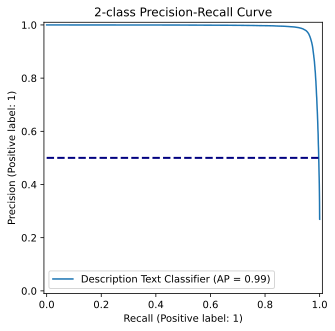
\includegraphics[width=0.475\textwidth]{figures/precision_recall_plot.pdf}
      \hfill
    %\vspace{-2cm}
    \includegraphics[width=0.475\textwidth]{figures/precision_recall_plot_extern.pdf}
\end{figure}
\end{frame}

%9
\begin{frame}
\frametitle{Classification Example I}
\begin{figure} [htbp]
    \centering
    %\vspace{-2cm}
    \includegraphics[width=\textwidth]{figures/web_crawler_example_sents_2.pdf}
\end{figure}
\end{frame}


%10
\begin{frame}
\frametitle{Classification Example II}
\begin{figure} [htbp]
    \centering
    %\vspace{-2cm}
    \includegraphics[width=\textwidth]{figures/web_crawler_example_sents_preds_2.pdf}
\end{figure}
\end{frame}



%11
\begin{frame}
\frametitle{And now?}
\begin{figure} [htbp]
    \centering
    %\vspace{-2cm}
    \includegraphics[width=\textwidth]{figures/web_crawler_example_sents_preds_2.pdf}
\end{figure}
\end{frame}

\end{document}


